% CREATED BY DAVID FRISK, 2016
\chapter{Introduction}
% remove lhc mentions because they acelerate protons?
\section{Conventional and plasma-wakefield accelerators}\vspace{-8pt}
%An estimated 30 000 particle accelerators are currently in operation worldwide, 
%forming an integral part of many areas of science and industry.
%providing beams of high-energy particles for science and industry. 

Ultra-relativistic electron beams with single-particle energies in excess of a GeV form an integral part of many areas of contemporary science, industry and medicine. 
For instance, monoenergetic electron bunches allows for the generation of high-quality X-ray pulses through the use of undulators; a technique by which ultra-relativistic electron bunches are rapidly oscillated back-and-forth perpendicular to their direction of propagation \cite{xfel}. This oscillatory motion can be tuned to generate highly coherent synchrotron radiation in the X-ray spectrum, which can be used in medicine for advanced tissue diagnostics, tomography and radiotheraphy cancer treatments \cite{Attwood}. Operating at higher energies, the 1.7 km long European X-ray free electron laser (XFEL) facility in Hamburg, Germany, employs 17.5 GeV electron bunches to generate extremely intense femtosecond X-ray pulses which are used for fundamental research into the structure of materials, biological molecules and even to generate movies of molecular reactions \cite{xfel}. Probing even smaller length scales takes us into the realm of high-energy electron-positron collider physics, where the size of accelerators grows accordingly. From the 3.2 km long, 45 GeV, SLAC Linear collider (SLC) at Stanford to the decommissioned 27 km long, 105 GeV, Large Electron Positron collider (LEP) at CERN, the fine details of the smallest constituents of our theories are being explored through tests of the standard model of particle physics. Even higher energy electron-positron colliders such as the proposed 50 km long International Linear Collider (ILC) aims to achieve single-particle energies up to 500 GeV. The reason for these progressively larger accelerators stems in part from the reliance on resonant radiofrequency (RF) cavities in order to accelerate particles, which are currently limited to sustaining electric fields no larger than$~100$MV/m, beyond which point further increase is hampered by material breakdown of the inner walls of the cavity \cite{Insepov2008}. As the demand for high-energy particle accelerators grows in medicine, industry and fundamental research, the size and cost of accelerators is and will continue to be a limit factor to future progress if no other means of acceleration is developed.\\
\indent Several novel accelerators techniques currently exists in various stages of development. The most widespread of these is based on the phenomena of \textit{plasma wakefield acceleration}. An ultra-relativistic particle beam or a high intensity laser pulses driven through a pre-formed plasma can excite plasma waves with phase velocities equal to the group velocity of the particle or laser driver \cite{Chen2002}. These waves, or 'wakefields', are large-amplitude oscillations of the plasma-electron density which are able to support accelerating electric fields of hundrends of GV/m; thousands of times higher than conventional RF cavities. By injecting an electron, or positron, bunch behind the driver one can then achieve constant acceleration by effectively letting the particle bunch surf the plasma-electron wave. In this manner, provided a sufficiently powerful driver is avilable, sizeable energy gains can be achieved over relatively short propgation distances. In fact, this form of plasma acceleration was proposed in 1979 by Tajima and Dawson \cite{Tajima1979}, not only as a viable terrestrial particle accelerator but also as a generation mechanism for ultra-high-energy cosmic rays in the plasma rich environment around newly formed pulsars. At the time of their proposal, however, the lack of sufficiently high intensity lasers was a limit factor in exploring these ideas experimentally \cite{Esarey2009}. The development of the chirped-pulse laser amplification techniques in 1985 by Strickland and Mourou \cite{Strickland1985} gave researchers access to ultrashort high-intensity laser pulses. This opened up the possibility of laser-driven plasma wakefield acceleration (LWFA) and several experiments constructed in the following decade were able to successfully demonstrate LWFA of electrons \cite{Clayton1993}. Recent experiments, propelled by the rapid development of modern multi-terawatt laser facilities, have demonstrated acceleration of electron bunches in a few centimetres of plasma up to 1, 2 and 4 GeV with relatively small energy spreads \cite{Leemans, Wang2013,  Leemans2014}, making LWFA a serious contender for the construction of compact x-ray free-electron lasers \cite{Huang2012}. Progress towards even higher energy gains have been made in the last two decades by the construction of dedicated beam-driven plasma wakefield acceleration (PWFA) facilities. Notably, experiments at the Facility for Advanced Accelerator Experimental Tests (FACET) at Stanford aims to use 20 GeV electron and positron beams to drive wakefields which in turn will accelerate secondary electron or positron bunches to higher energies \cite{Facet}. Furthermore, the Advanced Proton Driven Plasma Wakefield Acceleration Experiment (AWAKE) recently demonstrated proof-of-principle acceleration of secondary electron bunches up to 2 GeV within plasma wakefields driven by the 400 GeV proton beam from CERN’s Super Proton Synchrotron \cite{Adli2018}. These experiments are paving the way towards compact high-energy particle accelerators at GeV energies with great promise to science and industry. One can also imagine a future in which plasma wakefield accelerators are used in high-energy physics, perhaps in conjugation with conventional accelerators as a pre-accelerator or energy booster. Even though the latter is probably decades away, both GeV and TeV accelerators might still be able to benefit from plasma wakefield phenomena. Regardless of the means of acceleration, be it larger conventional accelerators or smaller plasma wakefield accelerators, the ultra-relativistic beams produced will need to be dealt with. The current approach for both small and large accelerators is to dump the energy of the beam. \vspace{-8pt}
\section{Beam dumps}\vspace{-8pt}
When in operation, the energy of the 105 GeV electron and positron beams at the LEP at CERN were dumped by directing them into a 2 m long, 40 cm in diameter, aluminium alloy block \cite{LEP_dump}. The proposed water-based beam dump for the ILC \cite{Satyamurthy2012}, which is to operate at 500 GeV, is significantly different to its lower energy predecessor at LEP. The increased energy and intensity of the ILC beam makes the extraction of its energy from a solid material beam dumps exceedingly difficult due to the limitations imposed by thermal conduction \cite{Satyamurthy2012}. By using a tank of water the ILC beam energy can be deposited and removed using a pumping system. However, the high intensity beams will lead to water temperatures in excess of 155\degree C as well as decomposition of water into hydrogen and oxygen gas. This necessitates a high-pressure vessel and a safe way to remove and store these violataile gases. Furthermore, the beam interaction with the water molecules will create the radioactive nuclei ${}^{3}$H and ${}^{7}$Be, which demands a waste-water storage tank. The tank itself will also suffer radiation damages, specifically the window through which the beam enters the vessel. A report by Satyamurthy et al. \cite{Satyamurthy2012} estimates that this window will need to be replaced at periodic intervals and due to the induced radioactivity this will have to be done remotely using robotic technology. Although this technology is widely available in the nuclear industry this whole beam dump is a large and costly affair for the ILC and any future HEP accelerators. Moreover, not only HEP accelerators face this issue, even metallic or concrete beam dumps for MeV to low GeV accelerators lead to radioactivation which must be carefully asses and adequately shielded for \cite{Schumann2009, Leuschner1998}. 



\begin{figure}
\centering
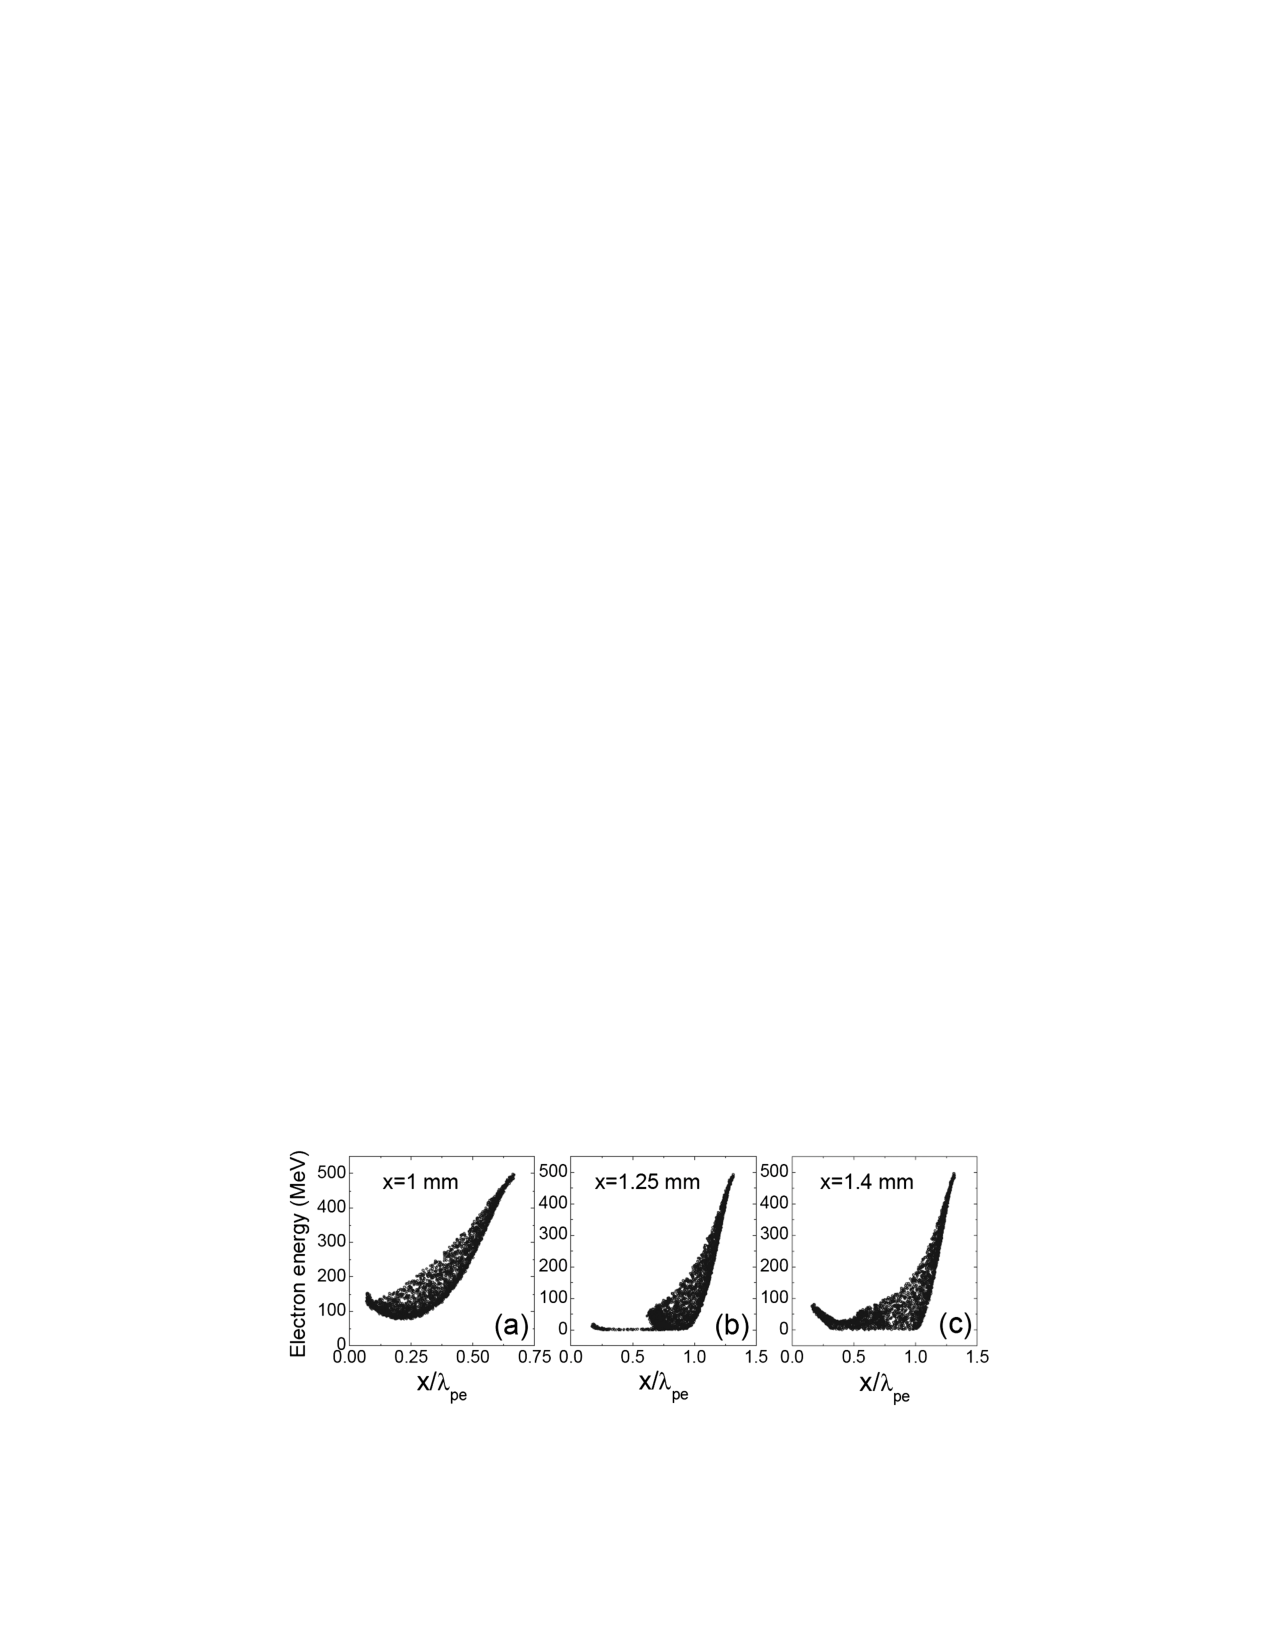
\includegraphics[width=0.9\textwidth]{Wu_energy_uniform.pdf}
\caption{\small{Energy distributions of an electron bunch during propagation through a dense plasma, as found by Wu et. al \cite{Wu2010}. 1(b) shows non-relativistic particles falling behind the head of the bunch and 1(c) shows their subsequently re-acceleration. The horizontal axis shows the distance along the bunch in relation to the plasma wavelength, which is covered in chapter 3.}}
\label{Wu}
\end{figure}
\indent An alternative approach aims to utilize the unprecedented acceleration gradients from PWFA. This idea, called a passive plasma beam dump, was proposed in 2010 by Wu et al. \cite{Wu2010}. They simulated a 500 MeV electron bunch and showed than an energy loss of up to 70\% was achievable by propagating 2 mm through a dense plasma, as shown in figure \ref{Wu}. Full energy depletion was prevented due to decelerated, non-relativistic, electrons falling behind behind the head of the bunch, figure 1(b), drifting into an accelerating region the wakefield and subsequently re-accelerated to relativistic energies, figure 1(c). This process prevents further significant energy loss and the deceleration is said to have saturated. It was further demonstrated that the decelerating field is independent of the initial bunch energy by demonstrating that a 100 GeV bunch would require $~20$ cm to loose 70\% of its energy \cite{Wu2010}. To minimize re-acceleration the simulated plasma was intersected by aerogel foils, strategically placed to capture the non-relativistic particles. This resulted in an energy loss of 90\% for the 500 MeV bunch. It is however not clear how prolonged exposure to plasma and interactions with high-energy electron bunches would affect the degradation of these foils. As an alternative, Hanahoe et al. \cite{Hanahoe2017} proposed the use of varying plasma density instead of foils. Linear or quadratically increasing plasma densities were shown to achieve comparable reduction of the re-accelerated particles as the foils used by Wu et al. It is however unclear whether such plasma density profiles can be set up and maintained in a plasma cell. 
Furthermore, the head of the bunch still maintained its energy in both these approaches; this \textit{energy chirp} is evident in figure 1(c) and occurs because the head of the bunch sets up the wakefield but does not experience the decelerating field itself \cite{Wu2010}. For the 500 MeV bunch this might not be a major issue since smaller conventional beam dumps could be used to dump this remaining energy. For GeV energies however this energy chirp may still pose an issue due to radioactivation. To address the energy chirp Bonatto et. al \cite{Bonatto2015} proposed the \textit{active beam dump}, whereby a laser pulse is driven ahead of the bunch through a plasma such that a decelerated wakefield is set up around the bunch. 
By carefully positioning the laser in relation to a 1 GeV bunch it was shown that the energy in the head of the bunch could be significantly reduced, resulting in total energy losses up to 95\%. It is however difficult to extend this method to higher energies due to the dispersion of the laser in the plasma, which prevents laser propagation over the longer distances required. \\
\indent Given that the active approach is able to reduce the energy chirp and that the passive beam dump leaves behind a pronounced energy chirp, the natural continuation of the previous work is to combine these methods. This project endeavours to demonstrate, through simulations, the successful combination of these methods in what we call a \textit{hybrid beam dump}. This scheme is outlined in figure \ref{hybrid_outline}.  The general approach is to use a passive beam dump to decelerate the bunch until saturation and then pass only the head of the bunch through an active beam dump, instead of decelerating the full-energy bunch with a laser driver as in the work by Bonatto et al.. This should have the added benefit of requiring a less powerful laser as well as being applicable to higher energies since previous work has shown that the energy chirp contains only $\sim 10\%$ of the initial energy. 






%The situation for its predecessor the LHC is similar, however the much larger energy carried by the protons requires a correspondingly larger beam dump. In this case, the 7 TeV proton beams are expanded and directed into a cylinder of graphite composite, 8 m long and 1 meter in diameter, which gets heated to 700\degree C upon impact and therefore contained in a water-cooled steel cylinder. This in turn, is encased in 750 tonnes of concrete and iron shielding [The LHC Beam Dumps website]. 


%Finally, Hanahoe et al. \cite{Hanahoe2017} proposed the use of varying plasma density instead of foils as an alternative way to prevent reaccelration. Linear or quadratically increasing plasma densities were shown to achieve comparable reduction of the reaccelrated particles as the foils used by Wu et al.  It is however unclear whether such plasma density profiles can be set up and sustained reliably in an experimental setting. \\


%Given that the passive beam dump schemes can dissipate a significant amount of energy with little technical difficulity, and that 

%With several proposed plasma beam dump techniques in place this project endeavours to merge the passive and active approaches in what we call a \textit{hybrid plasma beam dump}, with the goal of achieving a full energy depletion of the bunch. In addition, simulations will also be carried out for a recently approved plasma beam dump experiment at the FLASHForward facility at DESY in Germany. This will be the first dedicated plasma beam dump experiment of its kind and will be capable of testing both the passive and active approaches described above. 
\begin{figure}
\centering
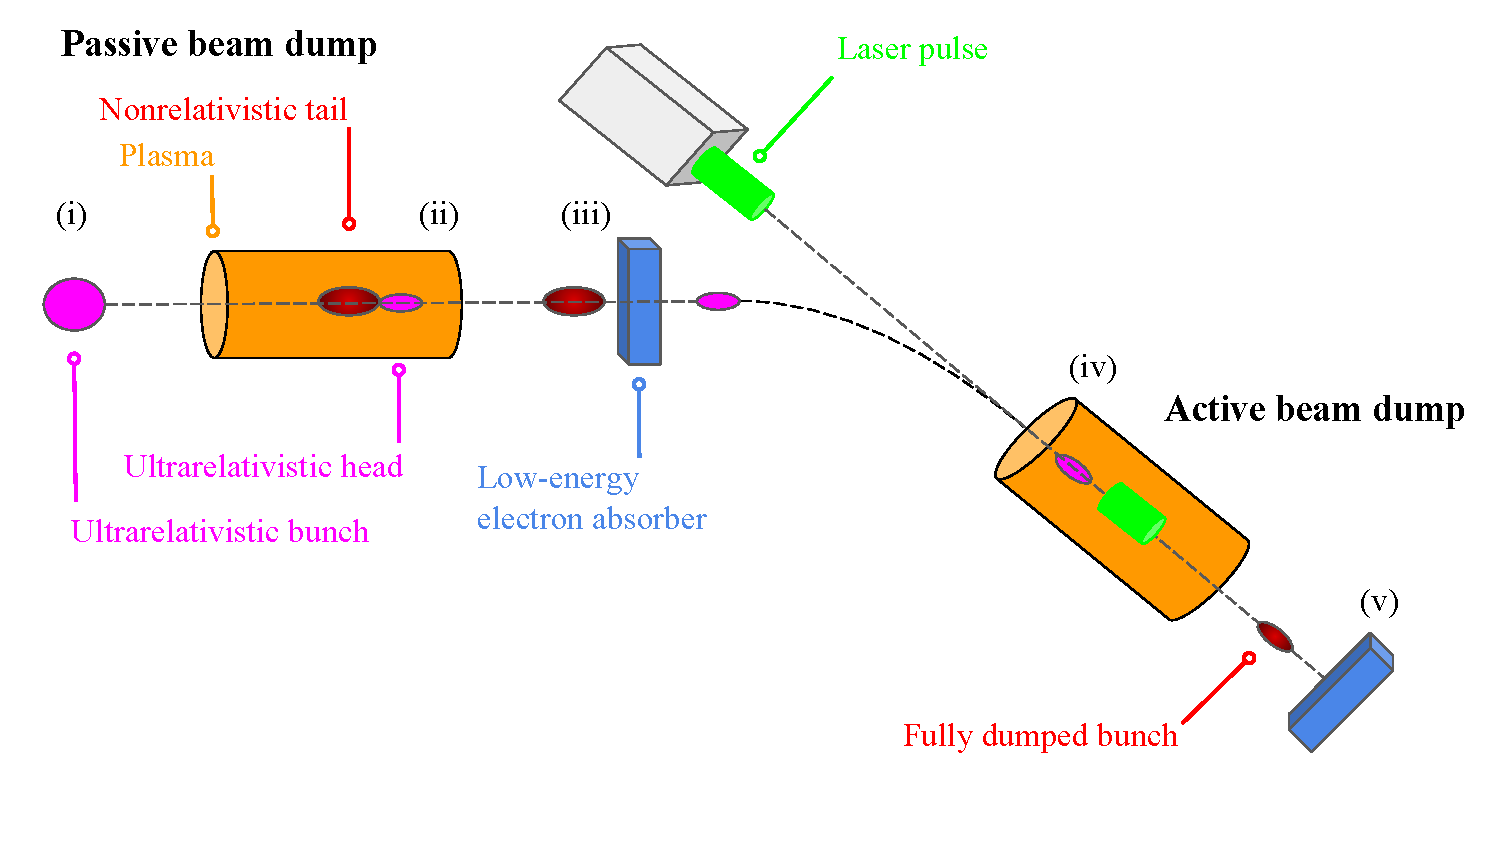
\includegraphics[width=\textwidth]{hybrid_outline5.pdf} %, expanding as it does so.
\caption{\small{Outline of the hybrid beam dump scheme at five stages. (i) The incoming ultra-relativistic (violet) electron bunch passes through vacuum towards the first plasma cell. (ii) The electron bunch loses energy as it propagates through the plasma. A non-relativistic (red) tail of particles is formed behind the the head of the bunch, which maintains its energy. (iii) The non-relativistic tail is removed by propagating through an absorbing material and the path of the head is bent by magnets so as to be aligned behind a laser pulse. (iv) The laser pulse drives a plasma wakefield in front of the remaining bunch, decelerating it to non-relativistic energies. (v) The remaining energy is absorbed.}} %%Alternatively, the tails is bent away by the magnets as well to avoid the head passing through and damaging the absorber material.
\label{hybrid_outline}
\end{figure}
\section{Outline of report}
This intermediate report details the initial phase of a full-year project on plasma wakefield deceleration and is written in partial fulfilment of the requirements for the degree of Master in Physics. As such, it does not attempt to cover the full scope of the work and research conducted in this project so far, but rather aims to provide and introduction to the field, establish the theoretical background and construct the computational framework necessary to perform the intended research. Having lain the groundwork for the project in this report, the the final-year report will reap the rewards of this work by presenting the full results and outcome of the project. \\
\indent Chapter 2 of this report details the simulation framework used in this project and  chapter 3 covers the theory behind beam-driven plasma wakefields. The theory describing laser-driven plasma wakefields, necessary to understand the active beam dump approach, will be covered in a subsequent report. Simulation tests and preliminary results are presented in chapter 4. We conclude this report by summarising the work that has been presented and looking ahead at the work that is to be carried out in the second half of this project.

%Superconduction RF (https://www.youtube.com/watch?v=HqrSb36QYVk)


%This restriction, together with the emission of synchrotron radiation in circular accelerators

%can sustain maximum electric fields 


%Full energy depletion was prevented by decelerated particles in the bunch reaching non-relativistic speeds and falling behind the main bunch, at which point they where picked up by the accelerating portion of the field and reaccelreated to realtivisitic speeds, the bunch energy is said to have saturated.

%To probe even smaller length scales the high-energy physics community relies on progressively larger accelerators.

%electric fields above 100 are hampered by material breakdown of the inner walls of the cavity \cite{Insepov2008}

%\indent The reason for this increase stems from the method by which particles are accelerated. High-energy particle accelerators rely on resonant radiofrequency (RF) cavities. 

%These are evacuated cavities which the particle beam passes through. The design and operation of these cavities are carefully engineered so as to set up an oscillating electric potential which acts to accelerate and squeeze the particle bunches together. 

%The current RF cavities at the LHC privde an accelerating field of 5MV/m, such that the energy gain per meter is 5MeV. 

%Hence, to reach TeV energies the protons at the LHC needs to pass through tens of millions RF cavities, which clearly necessitates a circular accelerator. The large size of the LHC then comes from the fact that the bending of the particles around the circular accelerator is limit by the magnetic field strength and the emission of synchrotron radiation.  [Add how much more energy LEP would have required to find the higgs]. Even if one used a combination of circular accellerators feed into a linear accelerator to avoid synchrotron energy loss, as in the proposed ILC, the size would still need to be large given that the maximum electric acceleration field in an RF cavity is $~$ 100MV/m, beyond which point....rf breakdown (seperation of ions and electrons). Clearly, even if the particle physics community is granted ever increasing particle accelerators, as the demand for GeV particle accelerators grows in medicine, industry and fundamental research, the size and cost of accelerators is and will continue to be a limit factor to future progress if no other means of acceleration is possible.\vspace{-8pt}